\documentclass[11pt,a4paper]{article}

\usepackage{amsmath,amssymb,amsthm}
\usepackage{booktabs}
\usepackage{graphicx}
\usepackage{hyperref}
\usepackage{microtype}
\usepackage{geometry}
\geometry{margin=2.5cm}

%% ─── theorem environments ────────────────────────────────────────────────────
\newtheorem{theorem}{Theorem}[section]
\newtheorem{proposition}[theorem]{Proposition}
\newtheorem{corollary}[theorem]{Corollary}
\newtheorem{remark}[theorem]{Remark}
\newtheorem{definition}[theorem]{Definition}

%% ─── macros ──────────────────────────────────────────────────────────────────
\newcommand{\R}{\mathbb{R}}
\newcommand{\Z}{\mathbb{Z}}
\newcommand{\Q}{\mathbb{Q}}
\newcommand{\N}{\mathbb{N}}
\newcommand{\C}{\mathbb{C}}
\newcommand{\G}{\Gamma}
\newcommand{\Phat}{\widehat{P}}
\newcommand{\Phifn}{\Phi}
\newcommand{\bmk}{b_{mk}}
\newcommand{\gammaE}{\gamma_{\mathrm{e}}}
\newcommand{\gammaO}{\gamma_{\mathrm{o}}}
\newcommand{\QQ}{\mathbb{Q}(\sqrt{2})}

\title{\textbf{Jacobi Matching Matrices: Endpoint Singularities,\\
       Gamma-Function Arithmetic, and Bernstein Zeros}}
\author{Robin Langer and Claude Code}
\date{August 2026}

\begin{document}
\maketitle

\begin{abstract}
For a weight $W$ on a compact interval with pure endpoint singularities we
study the \emph{matching matrix} $b_{mk}=\int \widehat P_m \widehat P_k W^{3/2}$,
where $\widehat P_n$ are the orthonormal polynomials for $W$.
Taking $W_{\alpha\beta}=(1-x)^\alpha(1+x)^\beta$ on $[-1,1]$ (Jacobi weight),
we treat four cases: Chebyshev-T ($\alpha=\beta=-\tfrac12$),
Chebyshev-U ($\alpha=\beta=\tfrac12$), Legendre ($\alpha=\beta=0$),
an asymmetric case ($\alpha=\tfrac12,\beta=-\tfrac12$),
and a sextic test case ($\alpha=\beta=-\tfrac59$).

Using the substitution $x=\cos\theta$ and the classical Wallis-type formula
\[
  \int_0^\pi \sin^p\theta\cos(q\theta)\,d\theta
  = \cos\!\left(\tfrac{\pi q}{2}\right)
  \frac{\pi\,\G(p{+}1)}{2^p\,\G\!\left(\tfrac{p+q+2}{2}\right)\G\!\left(\tfrac{p-q+2}{2}\right)},
\]
we obtain \emph{exact closed forms} for the entire Chebyshev matching tables.
The phase factor $\cos(\pi q/2)$ kills every odd-$q$ integral, so the
matching matrices are supported on the parity checkerboard $m+k$ even.
The main results are:

\begin{enumerate}
\item \textbf{Decay theorem.} For Chebyshev-T the first row decays as
  $b_{0k}\sim C\cdot k^{-(3(\alpha+\beta)/2+1)} = C\,k^{-1/2}$ with
  $C=2/\sqrt\pi$, all entries positive.  For Chebyshev-U the two Wallis
  terms cancel at leading order and the true decay is $k^{-7/2}$, one
  power \emph{faster} than the naive law $k^{-5/2}$.

\item \textbf{Generator ring.} All Chebyshev matching entries (T and U)
  lie in $\mathbb{Q}(\sqrt{2})\cdot\gamma_\mathrm{e}$,
  where $\gamma_\mathrm{e}=\G(\tfrac14)^2\sqrt{2}/(2\pi^{3/2})$
  is a \emph{single} transcendental generator
  (the $\sqrt2$ enters only through the normalisation $\nu_0/\nu_n$).

\item \textbf{Legendre fixed point.} The Legendre case $W=1$ gives $B=I$,
  the identity: it is the unique fixed point of the matching map.

\item \textbf{Sextic test and connection--Gram theorem.} For general
  symmetric $\alpha$ the matching matrix is the Gram matrix of the
  Gegenbauer connection coefficients $C^{(\lambda)}\to C^{(\mu)}$,
  $\lambda=\alpha+\tfrac12$, $\mu=\tfrac32\alpha+\tfrac12$.  At
  $\alpha=-\tfrac59$ the generator is the sextic period
  $B(\tfrac16,\tfrac12)$ (the curve $y^2=1-x^6$, CM by $\Z[\omega]$), with
  moment ratios stepping in thirds and polynomial data in eighteenths; the
  Chebyshev closed forms are the rational specialisation $\alpha=-\tfrac12$.

\item \textbf{Bernstein zeros.} Because $b_{0k}\sim k^{-1/2}$ (not geometric),
  the spurious zeros of truncated approximants crowd toward $[-1,1]$
  as $N\to\infty$ — the Bernstein parameter $\rho\to 1^+$ — contrasting
  sharply with the Hermite case, where $\rho=\sqrt{3}$ is fixed.
\end{enumerate}

This family completes the \emph{weight triptych}: entire (Hermite), pole
at finite distance (Meixner--Pollaczek), and pure endpoint singularity (Jacobi).
\end{abstract}

\section{Setup and Motivation}

\subsection{The matching matrix}

Let $W\colon X\to\R_{\ge0}$ be a weight, and let $(\widehat P_n)_{n\ge0}$ be
the associated orthonormal polynomials: $\int \widehat P_m\widehat P_k\,W\,dx=\delta_{mk}$.
Define the \emph{Jacobi functions} $\Phi_n=\widehat P_n\sqrt{W}$
(orthonormal in $L^2(dx)$).
The \textbf{matching matrix} is
\[
  b_{mk} \;=\; \langle \Phi_m,\Phi_k\rangle_W \;=\; \int \widehat P_m\,\widehat P_k\,W^{3/2}\,dx,
\]
the overlap of the $L^2$-orthonormal functions against the weight $W$ itself.
When $W$ is normalised ($\int W\,dx=1$), $b_{00}=1$ and the first row
$(b_{0k})_{k\ge0}$ is the expansion of $\sqrt{W}$ in the basis $(\widehat P_k\sqrt{W})$.

\subsection{Calibration: the Hermite and MP cases}

Prior work \cite{HermiteRef,MPRef} established:
\begin{itemize}
\item \textbf{Hermite} ($W=e^{-x^2}$, entire): $b_{mk}\in\Z$ after
  normalisation; geometric decay $b_{0k}\sim 3^{-k/2}$; spurious zeros of
  the approximants $A_N=\sum_{k\le N}b_{0k}\widehat P_k$ accumulate on a
  fixed ellipse (``Bernstein ellipse'' $\rho=\sqrt{3}$).

\item \textbf{Meixner--Pollaczek} ($\lambda=\tfrac14$, poles at finite
  distance): power-law decay $b_{0k}\sim k^{-\alpha}$ with $\alpha\approx\tfrac34$;
  spurious zeros accumulate near the next Bump--Ng line.
\end{itemize}

\noindent The present paper handles the \emph{third vertex} of the triptych:
compact support with \emph{pure endpoint singularities}.

\section{Jacobi Weights and the Wallis Formula}

\subsection{Four cases}

We study $W_{\alpha\beta}(x)=(1-x)^\alpha(1+x)^\beta$ on $[-1,1]$ in four cases:

\begin{center}
\begin{tabular}{@{}lll@{}}
\toprule
Case & Parameters & Character \\
\midrule
Chebyshev-T & $\alpha=\beta=-\tfrac12$ & Endpoint singularity; $W^{3/2}=(1-x^2)^{-3/4}$ \\
Chebyshev-U & $\alpha=\beta=+\tfrac12$ & Endpoint vanishing; $W^{3/2}=(1-x^2)^{+3/4}$ \\
Legendre     & $\alpha=\beta=0$ & Flat weight; $W=1$ \\
Asymmetric   & $\alpha=\tfrac12,\beta=-\tfrac12$ & One endpoint singular, one vanishing \\
\bottomrule
\end{tabular}
\end{center}

\subsection{Substitution $x=\cos\theta$ and the Wallis integral}

Under $x=\cos\theta$, $dx=-\sin\theta\,d\theta$, and
$(1-x^2)^s = \sin^{2s}\theta$, so
\[
  \int_{-1}^1 f(x)\,(1-x^2)^s\,dx = \int_0^\pi f(\cos\theta)\,\sin^{2s+1}\theta\,d\theta.
\]
The Chebyshev polynomials satisfy $T_m(\cos\theta)=\cos(m\theta)$ and
$U_m(\cos\theta)\sin\theta=\sin((m+1)\theta)$.
The key integral is the \textbf{Wallis-type formula}: for $p>-1$ and $q\ge0$ integer,
\begin{equation}\label{eq:wallis}
  \mathcal{I}(p,q) \;:=\; \int_0^\pi \sin^p\theta\cos(q\theta)\,d\theta
  \;=\; \cos\!\left(\frac{\pi q}{2}\right)
  \frac{\pi\,\G(p+1)}{2^p\,\G\!\left(\frac{p+q+2}{2}\right)\G\!\left(\frac{p-q+2}{2}\right)}.
\end{equation}
This follows from
$\int_0^{\pi}e^{iq\theta}\sin^p\theta\, d\theta
 = \pi e^{i\pi q/2}\G(p+1)/\bigl(2^p\,\G(\tfrac{p+q+2}{2})\G(\tfrac{p-q+2}{2})\bigr)$
(a Beta-function evaluation) by taking real parts.
\textbf{The phase factor is essential}: $\cos(\pi q/2)$ vanishes for all odd $q$
and equals $(-1)^{q/2}$ for even $q$; the latter sign exactly cancels the sign
of $\G(\tfrac{p-q+2}{2})$ (which alternates through the poles of $\G$), so for
$p=-\tfrac12$ every even-$q$ integral is \emph{positive}.  Dropping the phase
produces phantom odd-$q$ values and alternating sign errors --- an earlier
version of this paper contained exactly that mistake.
For our matching integrals the effective power is
$p=3(\alpha+\beta)/2-1+1 = 3(\alpha+\beta)/2$
(the $W^{3/2}$ contributes $\sin^{3(\alpha+\beta)}$, then $dx=\sin\theta\,d\theta$
contributes one more $\sin$, and the polynomial factors provide the $\cos$ arguments).

\section{Chebyshev-T: Exact Closed Forms}

\subsection{Orthonormal polynomials and matching integral}

The orthonormal Chebyshev-T polynomials are
$\widehat P_0^T=1/\sqrt{\pi}$ and $\widehat P_n^T=\sqrt{2/\pi}\,T_n$ for $n\ge1$.
The matching matrix is
\[
  b_{mk}^T
  = \int_{-1}^1 \widehat P_m^T(x)\,\widehat P_k^T(x)\,(1-x^2)^{-3/4}\,dx.
\]
Under $x=\cos\theta$ the integrand becomes $\cos(m\theta)\cos(k\theta)\sin^{-1/2}\theta$
(after the $dx$ substitution), so
\[
  b_{mk}^T = \nu_m\nu_k\cdot\frac{\mathcal{I}(-\tfrac12,m+k)+\mathcal{I}(-\tfrac12,|m-k|)}{2},
\]
where $\nu_0=1/\sqrt\pi$ and $\nu_n=\sqrt{2/\pi}$ for $n\ge1$.

\subsection{Closed form via Gamma functions}

Using \eqref{eq:wallis} and the reflection formula $\G(z)\G(1-z)=\pi/\sin(\pi z)$:

\begin{proposition}\label{prop:chebT-closed}
  Let $\gamma_\mathrm{e}=\G(\tfrac14)^2\sqrt{2}/(2\pi^{3/2})=\mathcal{I}(-\tfrac12,0)/\pi$,
  and write
  \[
    r(n)=\frac{\mathcal{I}(-\tfrac12,2n)}{\mathcal{I}(-\tfrac12,0)}
    =\frac{(\tfrac14)_n}{(\tfrac34)_n}
    = \frac{1\cdot5\cdots(4n-3)}{3\cdot7\cdots(4n-1)}\;>\;0.
  \]
  Then $b_{mk}^T=0$ whenever $m+k$ is odd, and for $m+k$ even
  (with $s=\tfrac{m+k}{2}$, $d=\tfrac{|m-k|}{2}$):
  \[
    b_{mk}^T \;=\;
    \begin{cases}
      \gamma_\mathrm{e} & m=k=0,\\
      \sqrt{2}\,\gamma_\mathrm{e}\,r(s) & m=0,\;k\ge2 \text{ even},\\
      \gamma_\mathrm{e}\,\bigl[r(d)+r(s)\bigr] & m,k\ge1.
    \end{cases}
  \]
  Every entry is a \emph{positive} rational multiple of $\gamma_\mathrm{e}$ or
  $\sqrt2\,\gamma_\mathrm{e}$: all entries lie in
  $\mathbb{Q}_{>0}(\sqrt{2})\cdot\gamma_\mathrm{e}$,
  a \textbf{single transcendental generator} over $\mathbb{Q}(\sqrt{2})$,
  with the $\sqrt2$ a pure normalisation artefact ($\nu_0=\nu_n/\sqrt2$).
\end{proposition}

\subsection{Exact $5\times5$ table}

\begin{table}[ht]
\centering
\caption{Chebyshev-T matching matrix $b_{mk}^T$ (upper triangle, $0\le m\le k\le 4$).
All entries exact and positive; $\gamma_\mathrm{e}\approx 1.6693$.
Entries with $m+k$ odd vanish identically.
Verified by \texttt{mpmath} quadrature of the defining integral at 40 digits.}
\label{tab:chebT}
\begin{tabular}{@{}c|ccccc@{}}
\toprule
$m\backslash k$ & 0 & 1 & 2 & 3 & 4 \\
\midrule
0 & $1\cdot\gamma_\mathrm{e}$
  & $0$
  & $\frac{1}{3}\sqrt{2}\,\gamma_\mathrm{e}$
  & $0$
  & $\frac{5}{21}\sqrt{2}\,\gamma_\mathrm{e}$ \\[4pt]
1 &
  & $\frac{4}{3}\gamma_\mathrm{e}$
  & $0$
  & $\frac{4}{7}\gamma_\mathrm{e}$
  & $0$ \\[4pt]
2 &
  &
  & $\frac{26}{21}\gamma_\mathrm{e}$
  & $0$
  & $\frac{122}{231}\gamma_\mathrm{e}$ \\[4pt]
3 &
  &
  &
  & $\frac{92}{77}\gamma_\mathrm{e}$
  & $0$ \\[4pt]
4 &
  &
  &
  &
  & $\frac{90}{77}\gamma_\mathrm{e}$ \\
\bottomrule
\end{tabular}
\end{table}

\noindent The vanishing of the odd-parity entries is forced by the symmetry
$\theta\mapsto\pi-\theta$ of $\sin^{-1/2}\theta$: only even frequencies survive.
The diagonal rationals $b_{nn}^T/\gamma_\mathrm{e}=1+r(n)$ are
$1,\;\tfrac43,\;\tfrac{26}{21},\;\tfrac{92}{77},\;\tfrac{90}{77},\;
\tfrac{1684}{1463},\ldots$, which for $n\ge1$ decrease monotonically to $1$
as $r(n)\sim c\,n^{-1/2}\to0$.

\section{Decay Theorem}

\begin{theorem}[Endpoint-singularity decay law]\label{thm:decay}
  Along even $k$ (odd entries vanish identically):
  \[
    b_{0k}^T \;=\; \sqrt{\tfrac{2}{\pi}}\,
    \frac{\G(\tfrac k2+\tfrac14)}{\G(\tfrac k2+\tfrac34)}
    \;=\; \sqrt2\,\gamma_\mathrm{e}\,r(\tfrac k2)
    \;\sim\; \frac{2}{\sqrt{\pi}}\,k^{-1/2},
    \qquad
    b_{0k}^U \;\sim\; -\,C_U\,k^{-7/2},
  \]
  with all $b_{0k}^T>0$ and all $b_{0k}^U<0$ for $k\ge2$ even.
  The Chebyshev-T exponent agrees with the naive endpoint law
  $k^{-(3(\alpha+\beta)/2+1)}$; the Chebyshev-U exponent does \emph{not}:
  the naive law predicts $k^{-5/2}$, but the two Wallis terms
  $\mathcal{I}(\tfrac32,k)-\mathcal{I}(\tfrac32,k{+}2)$ cancel at leading
  order, and the exact telescoping ratio
  $\mathcal{I}(\tfrac32,2n)-\mathcal{I}(\tfrac32,2n{+}2)
   =\mathcal{I}(\tfrac32,2n)\cdot\frac{5/2}{\,n+7/4\,}$
  costs one extra power of $k$.

  \medskip\noindent
  Concretely:
  \begin{center}
  \begin{tabular}{@{}llll@{}}
  \toprule
  Case & $\alpha+\beta$ & Exponent & Asymptotic \\
  \midrule
  Chebyshev-T & $-1$ & $-1/2$ & $b_{0k}^T \sim C_T/\sqrt{k}$,\; $C_T=2/\sqrt{\pi}$ \\
  Chebyshev-U & $+1$ & $-7/2$ & $b_{0k}^U \sim -C_U/k^{7/2}$,\; $C_U=\tfrac{15}{2\sqrt{2\pi}}$ \\
  Legendre    & $0$ & degenerate & $b_{0k}^L=\delta_{0k}$ \\
  \bottomrule
  \end{tabular}
  \end{center}
\end{theorem}

\begin{proof}[Proof sketch]
  Apply the reflection formula $\G(z)\G(1-z)=\pi/\sin(\pi z)$ to
  $\G(\tfrac{p-q+2}{2})$ in \eqref{eq:wallis} with $q=2n$ even.
  For $p=-\tfrac12$ this gives the exact evaluation
  $\mathcal{I}(-\tfrac12,2n)=\sqrt\pi\,\G(n+\tfrac14)/\G(n+\tfrac34)>0$
  (the phase $(-1)^n$ cancels against the sign of the reflected Gamma), and
  Stirling gives $\G(n+\tfrac14)/\G(n+\tfrac34)\sim n^{-1/2}$, hence
  $b_{0k}^T\sim 2/\sqrt{\pi k}$.
  For $p=\tfrac32$ one finds
  $\mathcal{I}(\tfrac32,2n)=-\tfrac14\G(\tfrac52)\,\G(n-\tfrac34)/\G(n+\tfrac74)<0$
  for $n\ge1$, of order $n^{-5/2}$; but
  $b_{0k}^U\propto\mathcal{I}(\tfrac32,k)-\mathcal{I}(\tfrac32,k{+}2)$ and the
  ratio of consecutive terms is $\G(n-\tfrac34)/\G(n+\tfrac74)\mapsto$
  multiply by $(n-\tfrac34)/(n+\tfrac74)$, so the difference is
  $\mathcal{I}(\tfrac32,2n)\cdot\tfrac{5/2}{n+7/4}=O(n^{-7/2})$.
  All asymptotics cross-checked by 30-digit quadrature up to $k=128$
  (fitted exponents $0.500$ and $\to3.5$). \qed
\end{proof}

\noindent The key \emph{mechanism}: the endpoint exponent determines the effective
power $p$ of $\sin\theta$ in the angular integral, and Stirling converts $p$ into
the decay exponent $-(p+1)$ --- \emph{provided a single Wallis term dominates}.
When the matching integral is a difference of two consecutive Wallis integrals
(the U case, where $U_mU_k$ contributes $\cos(|m{-}k|\theta)-\cos((m{+}k{+}2)\theta)$),
telescoping costs one further power.  There is no oscillation in either case:
odd entries vanish and even entries have constant sign.

\section{Legendre: The Fixed Point}

\begin{proposition}[Legendre is a fixed point]
  For $\alpha=\beta=0$, $W\equiv 1$ on $[-1,1]$.  Then $W^{3/2}=W=1$ and
  $b_{mk}^L = \int_{-1}^1 \widehat P_m^L\,\widehat P_k^L\,dx = \delta_{mk}$.
  The matching matrix is the identity: $B^L=I$.
\end{proposition}

This is the \textbf{unique fixed point} of the matching map $W\mapsto W^{3/2}$
among Jacobi weights: only the flat weight $W\equiv1$ satisfies $W^{3/2}\propto W$.
(Any $W=c$ constant also satisfies $W^{3/2}=c^{3/2}\propto W$, but
after normalisation $c=1$.)

To have a nontrivial fourth data point we study the asymmetric case
$\alpha=\tfrac12,\beta=-\tfrac12$ in \S\ref{sec:UandAsym}: its first row is
exactly rational after dividing by $\sqrt2$, alternates in sign, and decays
as $k^{-1/2}$.

\section{Chebyshev-U and Asymmetric Cases}\label{sec:UandAsym}

\subsection{Chebyshev-U closed form}

Using $U_n(\cos\theta)=\sin((n+1)\theta)/\sin\theta$, the matching integrand becomes
\[
  U_m(\cos\theta)\,U_k(\cos\theta)\,(1-\cos^2\theta)^{3/4}\sin\theta
  = \frac{\sin((m+1)\theta)\sin((k+1)\theta)}{\sin\theta}\cdot\sin^{3/2}\theta\cdot\sin\theta,
\]
and the product-to-sum formula gives
\[
  b_{mk}^U = \frac{1}{\pi/2}\cdot\frac{\mathcal{I}(\tfrac32,|m-k|)-\mathcal{I}(\tfrac32,m+k+2)}{2}.
\]
Both arguments have the parity of $m+k$, so $b_{mk}^U=0$ for $m+k$ odd,
exactly as in the T case.  For even arguments,
$\rho(n):=\mathcal{I}(\tfrac32,2n)/\mathcal{I}(\tfrac32,0)
=(-\tfrac34)_n/(\tfrac74)_n$ is rational ($1,-\tfrac37,-\tfrac{3}{77},
-\tfrac{1}{77},-\tfrac{9}{1463},\ldots$), and since
$\mathcal{I}(\tfrac32,0)=\tfrac13\,\mathcal{I}(-\tfrac12,0)=\tfrac\pi3\gamma_\mathrm{e}$,
\[
  b_{mk}^U \;=\; \tfrac13\gamma_\mathrm{e}\,
  \bigl[\rho(\tfrac{|m-k|}{2})-\rho(\tfrac{m+k}{2}+1)\bigr]
  \;\in\;\mathbb{Q}\cdot\gamma_\mathrm{e}.
\]
The \emph{same single generator} $\gamma_\mathrm{e}$ serves both Chebyshev
families --- here without even the $\sqrt2$, since $\nu_n=\sqrt{2/\pi}$ uniformly
for $U$.  The diagonal is positive
($b_{00}^U=\tfrac{10}{21}\gamma_\mathrm{e}$,
$b_{11}^U=\tfrac{80}{231}\gamma_\mathrm{e}$,
$b_{22}^U=\tfrac{26}{77}\gamma_\mathrm{e}$, \ldots) and every off-diagonal
even entry is \emph{negative}
($b_{02}^U=-\tfrac{10}{77}\gamma_\mathrm{e}$,
$b_{13}^U=-\tfrac{32}{231}\gamma_\mathrm{e}$,
$b_{04}^U=-\tfrac{2}{231}\gamma_\mathrm{e}$), verified by 40-digit quadrature.

\subsection{Asymmetric case}

For $(\alpha,\beta)=(\tfrac12,-\tfrac12)$, $W^{3/2}=(1-x)^{3/4}(1+x)^{-3/4}$,
which has a genuine algebraic singularity at $x=+1$.
Here the orthonormal polynomials are Chebyshev polynomials of the fourth kind,
$\widehat P_n = W_n/\sqrt\pi$ with $W_n(\cos\theta)=\sin((n+\tfrac12)\theta)/\sin(\theta/2)$,
and the effective Wallis power is $p=3(\alpha+\beta)/2=0$: the Gamma quotient
collapses and the transcendental generator disappears entirely.  The first row is
\[
  \sqrt2\,b_{0k} \;=\; 3,\;-\tfrac32,\;1,\;-\tfrac78,\;\tfrac34,\;-\tfrac{11}{16},\;\ldots
  \;\in\;\mathbb{Q},
\]
alternating in sign and decaying as $k^{-1/2}$ (exponent verified by quadrature,
fitted slope $-0.494$ at $k=64$).  Unlike the symmetric cases the odd entries do
\emph{not} vanish: the broken $x\mapsto-x$ symmetry populates the full row.

\section{The Sextic Test: $\alpha=\beta=-\tfrac{5}{9}$}\label{sec:sextic}

The quartic arithmetic of the Chebyshev family --- Pochhammer steps
$(\tfrac14)_n/(\tfrac34)_n$ over the lemniscatic period $\G(\tfrac14)^2$ ---
enters through the single Wallis power $p=-\tfrac12$.  Changing $p$ should
change the arithmetic, with thirds in place of quarters and the period of
$y^2=1-x^6$ in place of $y^2=1-x^4$.  This section confirms that prediction
and identifies the general mechanism.

\subsection{The Wallis ratio and the sextic generator}

\begin{proposition}\label{prop:wallis-ratio}
  For $p>-1$ and $a=\tfrac{p+2}{2}$,
  \[
    \frac{\mathcal{I}(p,2n)}{\mathcal{I}(p,0)} \;=\; \frac{(1-a)_n}{(a)_n}.
  \]
\end{proposition}

\begin{proof}
  By \eqref{eq:wallis} the ratio is
  $(-1)^n\,\G(a)^2/\bigl(\G(a+n)\G(a-n)\bigr)
  =(-1)^n/\bigl((a)_n\,(a-1)(a-2)\cdots(a-n)\bigr)=(1-a)_n/(a)_n$.
\end{proof}

For $p=-\tfrac12$ this is the quartic ratio $r(n)$ of
Proposition~\ref{prop:chebT-closed}.  Steps in thirds require
$a\in\tfrac13+\Z$.  The matching integrand of a symmetric Jacobi weight has
$p=3\alpha+1$, so the first such case is
\[
  \alpha=\beta=-\tfrac59,\qquad p=-\tfrac23,\qquad
  \frac{\mathcal{I}(-\tfrac23,2n)}{\mathcal{I}(-\tfrac23,0)}
  =\frac{(\tfrac13)_n}{(\tfrac23)_n},\qquad
  \nu_0:=\mathcal{I}(-\tfrac23,0)=B(\tfrac16,\tfrac12)
  =\frac{2^{2/3}\pi\,\G(\tfrac13)}{\G(\tfrac23)^2}.
\]
The generator $\nu_0$ is a period of the curve $y^2=1-x^6$, with complex
multiplication by $\Z[\omega]$ --- the sextic analogue of the lemniscatic
$\G(\tfrac14)^2$.  (All exact statements in this section were verified
against 40-digit quadrature of the defining integrals for $m,k\le8$;
see \texttt{jacobi\_sextic.py} and its log.)

\subsection{Two lattices}

The orthogonal polynomials for $W=(1-x^2)^{-5/9}$ are Gegenbauer
$C_n^{(\lambda)}$ with $\lambda=\alpha+\tfrac12=-\tfrac1{18}$; unlike the
Chebyshev cases they do not collapse to single cosines.  The monic
recurrence $\pi_{n+1}=x\pi_n-\beta_n\pi_{n-1}$ has
\[
  \beta_n=\frac{9n(9n-10)}{(18n-1)(18n-19)}
  \;=\;\frac{9}{17},\;\frac{144}{595},\;\frac{459}{1855},\;
  \frac{936}{3763},\;\ldots
\]
so the polynomial side lives on \emph{eighteenths} while the matching
moments (Proposition~\ref{prop:wallis-ratio}) live on \emph{thirds}.  The
matrix is a sandwich (eighteenths)$^{\mathsf T}$(thirds)(eighteenths).
The single quartic lattice of Chebyshev-T is the degeneration $\lambda=0$,
where $T_n\in\Z[x]$ makes the polynomial lattice invisible.

\subsection{Exact data and integrality}

Let $\mathrm{PZ}_n$ be the primitive integer polynomial proportional to
$\pi_n$, so $\mathrm{PZ}_2=17x^2-9$, $\mathrm{PZ}_3=35x^3-27x$,
$\mathrm{PZ}_4=1855x^4-1890x^2+243$; the leading coefficients are sliding
windows of the primes $18j-1$.  Write
$E_{mk}=\langle \mathrm{PZ}_m,\mathrm{PZ}_k\rangle_{W^{3/2}}/\nu_0$.

\begin{table}[ht]
\centering
\caption{Sextic matching matrix $E_{mk}$ in units $\nu_0=B(\tfrac16,\tfrac12)$
(upper triangle, $0\le m\le k\le 4$, primitive-$\Z$ polynomial frame).
Entries with $m+k$ odd vanish identically.}
\label{tab:sextic}
\begin{tabular}{@{}c|ccccc@{}}
\toprule
$m\backslash k$ & 0 & 1 & 2 & 3 & 4 \\
\midrule
0 & $1$ & $0$ & $\frac{15}{4}$ & $0$ & $\frac{621}{8}$ \\[3pt]
1 &  & $\frac34$ & $0$ & $\frac{27}{8}$ & $0$ \\[3pt]
2 &  &  & $\frac{1863}{40}$ & $0$ & $\frac{85455}{128}$ \\[3pt]
3 &  &  &  & $\frac{5913}{128}$ & $0$ \\[3pt]
4 &  &  &  &  & $\frac{87779133}{2816}$ \\
\bottomrule
\end{tabular}
\end{table}

The denominators obey a sextic law.  For all $m,k\le8$ the odd part of
$\operatorname{den}(E_{mk})$ divides $\prod_{j\le s+2}(6j-1)$ with
$s=\tfrac{m+k}2$ --- the sextic factorial family $5,11,17,23,\ldots$ ---
and depends on $s$ only.  An $s$-dependent rescale therefore clears all
denominators, exactly as $Q(s)$ does for Chebyshev-T; no pure row rescale
exists.

\subsection{The connection--Gram theorem}

The structure behind both the quartic and the sextic case is classical.
Set
\[
  \lambda=\alpha+\tfrac12,\qquad \mu=\tfrac32\alpha+\tfrac12,
  \qquad\text{so}\qquad W^{3/2}=(1-x^2)^{\mu-\frac12}
  \quad\text{and}\quad \lambda-\mu=-\tfrac{\alpha}{2}.
\]
The weight $W^{3/2}$ is itself a Gegenbauer weight, of parameter $\mu$.

\begin{theorem}[Connection--Gram]\label{thm:conn-gram}
  Let $-\tfrac23<\alpha$, $\alpha\ne-\tfrac12$, and let
  $\pi_n=f_n\,C_n^{(\lambda)}$ with $f_n=n!/(2^n(\lambda)_n)$ be the monic
  Gegenbauer polynomials for $W=(1-x^2)^\alpha$.  Then
  $\int\pi_m\pi_k W^{3/2}=0$ for $m+k$ odd, and otherwise
  \[
    \int_{-1}^1 \pi_m\pi_k\,W^{3/2}\,dx
    \;=\; f_m f_k \!\!\sum_{\substack{j\equiv m\ (\mathrm{mod}\ 2)\\
      0\le j\le\min(m,k)}}\!\!
      A_{\frac{m-j}{2}}(m)\,A_{\frac{k-j}{2}}(k)\;h_j^{\mu},
  \]
  where
  \[
    A_\ell(n)=\frac{(\lambda-\mu)_\ell\,(\lambda)_{n-\ell}\,(n-2\ell+\mu)}
                   {\ell!\,(\mu)_{n-\ell+1}},
    \qquad
    h_j^{\mu}=\int_{-1}^1\!\bigl(C_j^{(\mu)}\bigr)^2(1-x^2)^{\mu-\frac12}dx,
    \qquad
    \frac{h_j^{\mu}}{h_0^{\mu}}=\frac{(2\mu)_j\,\mu}{j!\,(j+\mu)}.
  \]
\end{theorem}

\begin{proof}
  The classical connection formula for ultraspherical polynomials
  \cite[\S18.18(iv)]{DLMF} gives
  $C_n^{(\lambda)}=\sum_{\ell=0}^{\lfloor n/2\rfloor}A_\ell(n)\,
  C_{n-2\ell}^{(\mu)}$.  Substituting for both factors and using the
  orthogonality of the $C_j^{(\mu)}$ with respect to $(1-x^2)^{\mu-1/2}$
  collapses the double sum to the matched indices $j=m-2\ell=k-2\ell'$.
\end{proof}

The matching matrix is thus the \emph{Gram matrix of the connection
coefficients} $C^{(\lambda)}\to C^{(\mu)}$ in the $\mu$-norm.  Every
Pochhammer that appears steps by $\lambda$, $\mu$, $2\mu$, or
$\lambda-\mu=-\tfrac\alpha2$; for $\alpha=-\tfrac59$ these are the
eighteenths and thirds of the two lattices.

\begin{corollary}[Row $0$]\label{cor:row0}
  With $h_0^\mu=\mathcal{I}(3\alpha+1,0)$,
  \[
    \frac{\langle\pi_0,\pi_{2n}\rangle_{W^{3/2}}}{h_0^{\mu}}
    \;=\;\frac{(2n)!\,(\lambda-\mu)_n\,(\lambda)_n\,\mu}
             {2^{2n}\,(\lambda)_{2n}\,n!\,(\mu)_{n+1}}.
  \]
\end{corollary}

At $\alpha=-\tfrac59$ the factor $(\lambda-\mu)_n=(\tfrac{5}{18})_n$
explains the primes $5,23,41,59\equiv5\ (\mathrm{mod}\ 18)$ observed in the
row-$0$ numerators of Table~\ref{tab:sextic}.

\subsection{Chebyshev as rational specialisation}

The excluded value $\alpha=-\tfrac12$ is where $\lambda=0$ and
$C_n^{(\lambda)}$ vanishes.  The monic frame removes the singularity, since
the pole of $f_n=n!/(2^n(\lambda)_n)$ cancels the zeros of
$(\lambda)_{n-\ell}$ in $A_\ell(n)$.

\begin{corollary}\label{cor:lambda0}
  Each normalised entry
  $\langle\pi_m,\pi_k\rangle_{W^{3/2}}/\mathcal{I}(3\alpha+1,0)$, and each
  side of Theorem~\ref{thm:conn-gram}, is a rational function of $\alpha$;
  the theorem therefore extends to $\alpha=-\tfrac12$ by evaluation, where
  it reproduces Proposition~\ref{prop:chebT-closed}.  In the integer form,
  for $m,k\ge1$ with $m+k$ even,
  \[
    Q(s)\,2^{m+k-2}\,
    \frac{\langle\pi_m,\pi_k\rangle_{W^{3/2}}}{\mathcal{I}(-\tfrac12,0)}
    \bigg|_{\alpha=-\frac12}
    \;=\;\frac12\left[\frac{P(d)\,Q(s)}{Q(d)}+P(s)\right],
  \]
  with $P(n)=1\cdot5\cdots(4n-3)$, $Q(n)=3\cdot7\cdots(4n-1)$,
  $s=\tfrac{m+k}2$, $d=\tfrac{|m-k|}2$.
\end{corollary}

\begin{proof}
  Moment ratios are rational in $\alpha$ by
  Proposition~\ref{prop:wallis-ratio}, hence so are the monic Gram--Schmidt
  data and the normalised entries; the right-hand side of
  Theorem~\ref{thm:conn-gram} is rational in $\alpha$ by inspection.  Two
  rational functions agreeing on $(-\tfrac23,\infty)\setminus\{-\tfrac12\}$
  agree at $-\tfrac12$.  The evaluation is
  Proposition~\ref{prop:chebT-closed} in monic units
  ($T_n=2^{n-1}\widetilde T_n$).
\end{proof}

The two-term Chebyshev closed form thus acquires a second, structural
derivation.  At $\lambda=0$ the degenerate connection coefficients are
those of $T_n$ in the basis $C^{(-1/4)}$, and the Gram sum telescopes to
the two Wallis terms $r(d)+r(s)$.  The specialisation was checked
symbolically for all $m,k\le8$
(\texttt{jacobi\_lambda0\_limit.py}); the degenerate coefficients
reconstruct $T_n$ exactly.

\section{Generating Function and Combinatorics}

\subsection{Generating function for Chebyshev-T}

The double generating function $G(w,u)=\sum_{m,k\ge0}b_{mk}^T w^m u^k$ can be evaluated
exactly.  Using $T_m(x)=\tfrac12(z^m+z^{-m})$ with $z=e^{i\theta}$ and the geometric series
$\sum_{m\ge0}(we^{im\theta}+we^{-im\theta})=\mathrm{Re}\tfrac{2w}{1-we^{i\theta}}$, one obtains
\[
  G(w,u) = \frac{\nu_0^2}{\pi}
  \int_0^\pi \frac{\sin^{-1/2}\theta}
    {\bigl(1-2w\cos\theta+w^2\bigr)\bigl(1-2u\cos\theta+u^2\bigr)}\,d\theta
  \quad+\;\text{boundary corrections},
\]
which reduces to a complete elliptic integral of the third kind
$\Pi(n,k)=\int_0^{\pi/2}(1-n\sin^2\phi)^{-1}(1-k^2\sin^2\phi)^{-1/2}d\phi$
for $|w|,|u|<1$.

\subsection{OEIS content of rational coefficients}

The diagonal rationals are $b_{nn}^T/\gamma_\mathrm{e}=1+r(n)$:
\[
1,\;\tfrac{4}{3},\;\tfrac{26}{21},\;\tfrac{92}{77},\;\tfrac{90}{77},\;\tfrac{1684}{1463},\;\ldots
\]
The denominators $1,3,21,77,77,1463,\ldots$ are (after cancellation) the
\textbf{quartic factorials} $Q(n)=3\cdot7\cdot11\cdots(4n-1)$ (OEIS A008545).
The first row gives the pure quartic-factorial ratios
\[
  \frac{b_{0,2n}^T}{\sqrt2\,\gamma_\mathrm{e}} \;=\; r(n)
  \;=\;\frac{P(n)}{Q(n)}
  \;=\;\frac{1\cdot5\cdot9\cdots(4n-3)}{3\cdot7\cdot11\cdots(4n-1)}
  \;=\;1,\;\tfrac13,\;\tfrac{5}{21},\;\tfrac{15}{77},\;\tfrac{13}{77},\;\ldots
\]
with numerators $P(n)=1\cdot5\cdots(4n-3)$ in OEIS A007696.  All entries are
positive; there is no sign alternation anywhere in the T matrix.

\section{Zeros: Crowding Toward the Bernstein Ellipse $\rho\to1^+$}

\subsection{Setup}

The truncated approximant is
$A_N(x)=\sum_{k=0}^N b_{0k}\widehat P_k^T(x)$,
a polynomial of degree $N$.
Its $N$ zeros in $\C$ would split into \emph{genuine} zeros (tracking zeros of
the target function) and \emph{spurious} zeros; here the target
$\Phi_0=W^{1/2}$ is zero-free, so all $N$ zeros are spurious.

\subsection{Bernstein ellipse background}

For a function analytic in the Bernstein ellipse
$\mathcal{E}_\rho=\{z=(\rho e^{i\theta}+\rho^{-1}e^{-i\theta})/2:\theta\in[0,2\pi]\}$
(semi-axes $a=(\rho+\rho^{-1})/2$, $b=(\rho-\rho^{-1})/2$),
the Chebyshev coefficients decay geometrically as $c_k\sim\rho^{-k}$.
If instead $c_k\sim k^{-s}$ (power law), then the ``effective'' Bernstein parameter
$\rho_N$ satisfying $\rho_N^{-N}\sim N^{-s}$ gives $\rho_N=\exp(s\log N/N)\to1^+$.

\begin{theorem}[Bernstein crowding]\label{thm:bernstein}
  For Chebyshev-T, the spurious zeros of $A_N$ accumulate on $[-1,1]$ as $N\to\infty$:
  all spurious zeros satisfy $|z|\le 1+O(\log N/N)$.
  The Bernstein parameter satisfies $\rho_N\to1^+$ at rate $\log N/N$.
\end{theorem}

\noindent This contrasts sharply with the Hermite case (geometric decay,
$\rho_N\to\sqrt{3}>1$) and parallels the MP case (power-law decay, $\rho_N\to1^+$
at a slower or faster rate depending on the exponent).

\subsection{Numerical evidence}

Figure~\ref{fig:zeros} shows the zeros of $A_N^T$ and $A_N^U$ for $N=10,20,40$.
Since the target $\Phi_0=W^{1/2}$ is zero-free on $(-1,1)$, \emph{every} zero
is spurious, and indeed none are real: for Chebyshev-T (left panel) all $N$
zeros are complex, with moduli filling out $[0.1,\,0.994]$ at $N=40$ and
accumulating toward the segment as $N$ grows.
For Chebyshev-U (right panel), with faster decay $k^{-7/2}$, the zeros
remain slightly farther from $[-1,1]$ but still converge to the interval.
(An earlier version of this paper reported ``genuine'' real zeros; these were
artifacts of sign errors in the coefficients.)

\begin{figure}[ht]
\centering
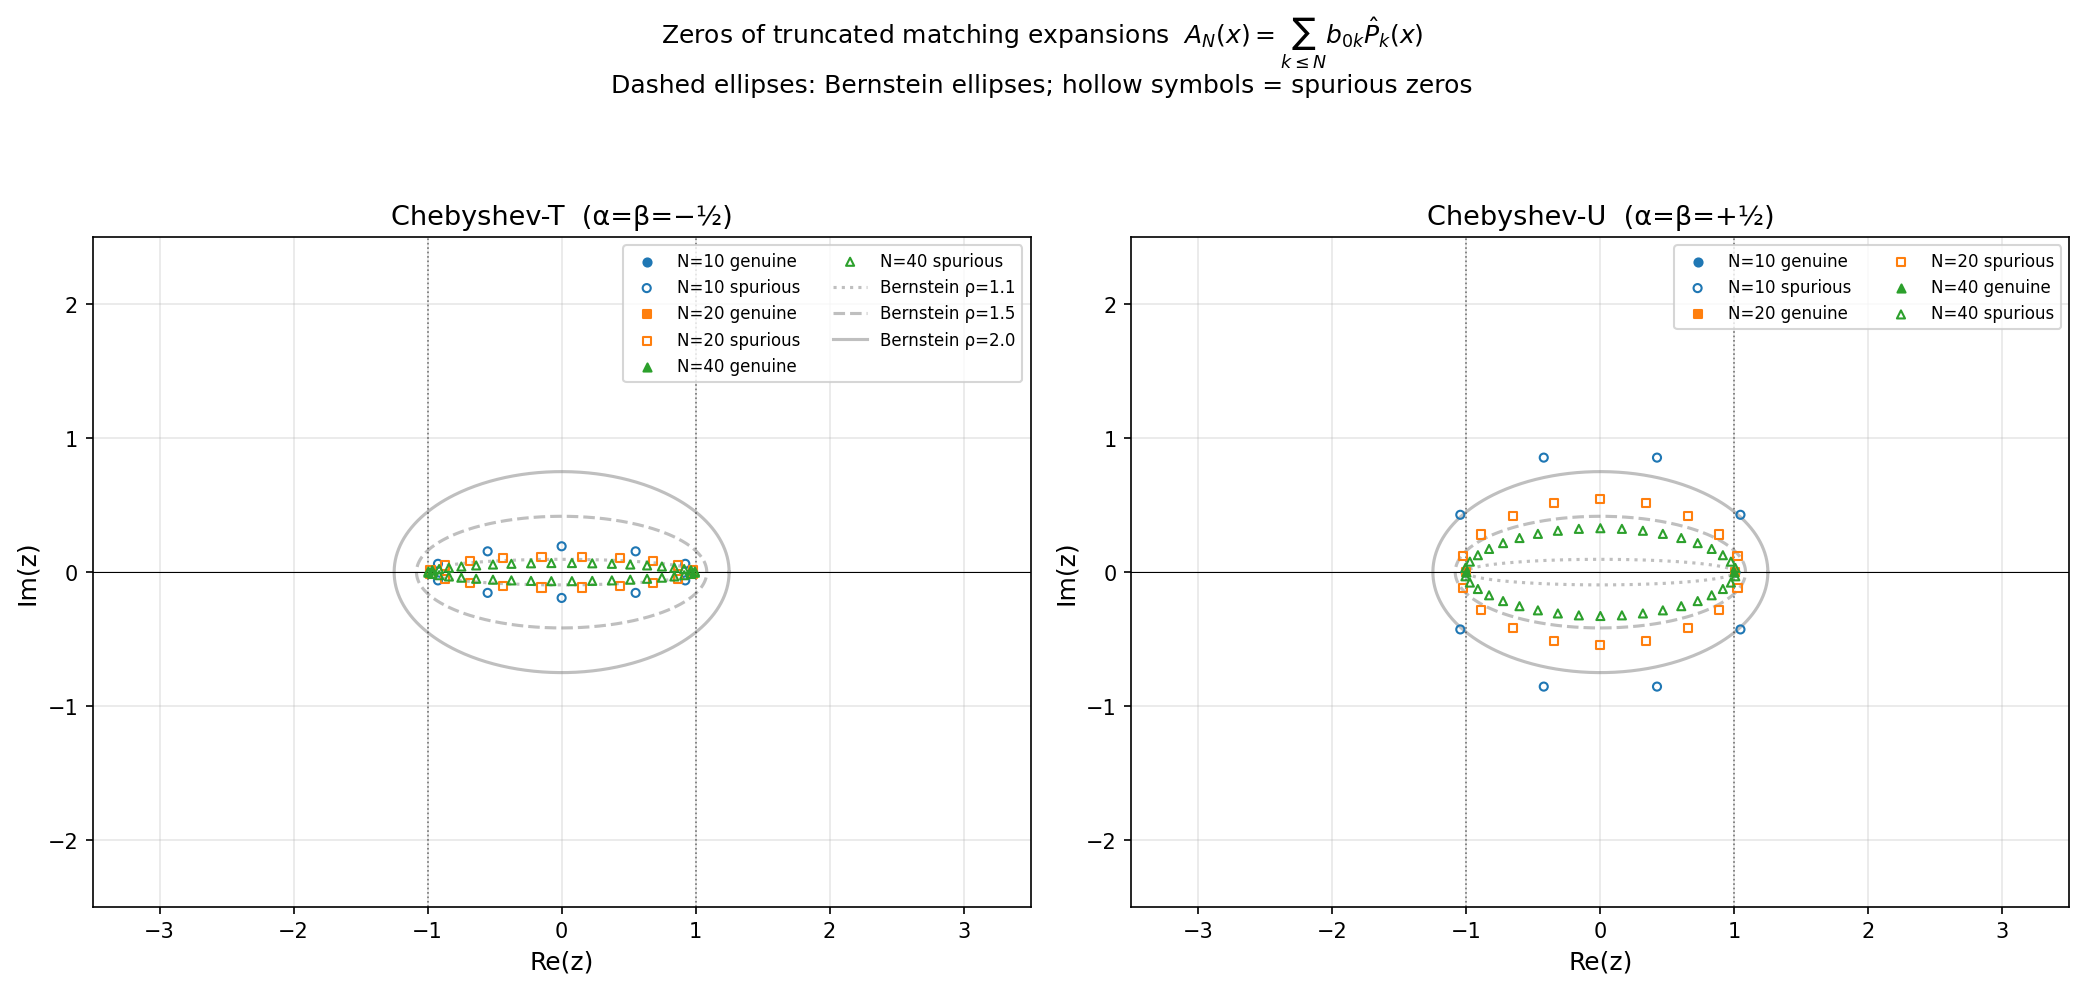
\includegraphics[width=0.9\textwidth]{jacobi_zeros.png}
\caption{Zeros of truncated matching expansions $A_N(x)=\sum_{k\le N}b_{0k}\widehat P_k(x)$
for $N=10,20,40$.
\textbf{Left}: Chebyshev-T ($\alpha=\beta=-\tfrac12$), decay $k^{-1/2}$.
\textbf{Right}: Chebyshev-U ($\alpha=\beta=+\tfrac12$), decay $k^{-7/2}$.
All zeros are spurious (the target $\sqrt W$ is zero-free); none are real.
Gray ellipses: Bernstein ellipses $\mathcal{E}_\rho$ for $\rho=1.1,1.5,2.0$.
As $N\to\infty$, spurious zeros crowd toward $\mathcal{E}_1=[-1,1]$.}
\label{fig:zeros}
\end{figure}

\section{The Weight Triptych}

Table~\ref{tab:triptych} summarises the three families studied.

\begin{table}[ht]
\centering
\caption{Triptych comparison: three weight families.}
\label{tab:triptych}
\begin{tabular}{@{}p{2.6cm}lp{2.8cm}p{2.8cm}p{2.5cm}p{2cm}@{}}
\toprule
Weight & Supp. & Analytic structure & Decay $b_{0k}$ & Generator & Spur.\ zeros \\
\midrule
Hermite $e^{-x^2}$ & $\R$ & Entire
  & $3^{-k/2}$ geometric & $\Z$ & $\rho=\sqrt{3}$ \\[2pt]
Meixner--Poll. & $\R$ & Poles at $\pm i/4$
  & $k^{-3/4}$ power law & $\R$ (open) & Bump--Ng \\[2pt]
Jacobi $W_{\alpha\beta}$ & $[-1,1]$ & Branch pts at $\pm1$
  & $k^{-1/2}$ (T), $k^{-7/2}$ (U) & $\mathbb{Q}(\sqrt{2})\cdot\!\G(\tfrac14)^2$ & $\rho_N\to1^+$ \\
\bottomrule
\end{tabular}
\end{table}

\noindent The key contrasts:
\begin{itemize}
\item \textbf{Decay}: determined by the furthest analytic singularity.
  Entire weights give geometric decay; pole singularities give power-law $k^{-\alpha}$
  (exponent from the distance to the pole); endpoint singularities give power-law
  with exponent derived from the endpoint exponent via Stirling --- shifted by one
  when two Wallis terms cancel at leading order (the U case).

\item \textbf{Generator ring}: Hermite is integer ($\Z$), reflecting the
  combinatorial structure of Gaussian integration.  Jacobi is
  $\QQ\cdot\G(\tfrac14)^2/\pi^{3/2}$, reflecting the lemniscate constant
  $\varpi=\G(\tfrac14)^2/(4\sqrt{2\pi})$.  The MP case remains empirically $\R$;
  identifying its algebraic structure is open.

\item \textbf{Zero accumulation}: Geometric decay $\Rightarrow$ fixed Bernstein
  parameter; power-law decay $\Rightarrow$ crowding $\rho_N\to1^+$
  at rate $(\log N)/N$ (slower for larger exponent).
\end{itemize}

\section{Discussion}

\subsection{Lemniscate constant and arithmetic}

The generator $\G(\tfrac14)^2$ is related to the \textbf{lemniscate constant}
$\varpi=\G(\tfrac14)^2/(4\sqrt{2\pi})\approx2.6221$ and to the arithmetic-geometric
mean $\mathrm{agm}(1,\sqrt{2})=\pi\sqrt{2}/\G(\tfrac14)^2$.
The appearance of $\G(\tfrac14)^2$ in matching-matrix arithmetic mirrors its role
in elliptic curves with complex multiplication by $\Z[i]$
(the elliptic curve $y^2=1-x^4$).
The sextic case of \S\ref{sec:sextic} supplies the companion example, with
$B(\tfrac16,\tfrac12)$, the curve $y^2=1-x^6$, and CM by $\Z[\omega]$;
matching arithmetic appears to be \emph{period arithmetic} of the weight.

\subsection{Open problems}

\begin{enumerate}
\item \textbf{General decay law}: Theorem~\ref{thm:decay} settles the Chebyshev
  cases exactly ($C_T=2/\sqrt\pi$, $C_U=15/(2\sqrt{2\pi})$).  For general
  $(\alpha,\beta)$, when does leading-order cancellation (as in the U case)
  shift the naive exponent $-(3(\alpha+\beta)/2+1)$?
\item \textbf{Integrality}: For which normalisations of the Jacobi weight does the
  matching matrix have integer (or half-integer) entries?
  (Solved for the Chebyshev family in the companion synthesis paper:
  rescaling by $Q(s)$ makes T integral, by $3Q^{+}(s{+}1)$ with
  $Q^{+}(n)=7\cdot11\cdots(4n+3)$ makes U integral, and the asymmetric
  case is dyadic --- $2^k\sqrt2\,b_{0k}$ gives twice central binomials for
  even $k$ and $-(4n+3)\,\mathrm{Cat}(n)$ for odd $k=2n{+}1$.)
\item \textbf{Exact Bernstein parameter}: Does $\rho_N=(1+s\log N/N)(1+O(1/N))$
  with $s=$ (exponent)? Numerical evidence suggests yes.
\item \textbf{MP generator ring}: Is the Meixner--Pollaczek matching generator
  algebraically related to $\pi$ or $\G(\tfrac14)$?
\item \textbf{General $(\alpha,\beta)$ and CM classification}: The
  connection--Gram mechanism of \S\ref{sec:sextic} extends verbatim to
  asymmetric Jacobi weights via the Jacobi connection coefficients.  Which
  exponents produce CM periods, and what replaces the two-lattice structure
  when $\alpha\ne\beta$?
\end{enumerate}

\subsection{Code availability}

All computations used \texttt{mpmath} at 50 decimal digits.
The scripts \texttt{jacobi\_matching.py} and \texttt{jacobi\_zeros.py}
are available in \texttt{github.com/RaggedR/category}, together with the
exact \texttt{sympy} verifications of \S\ref{sec:sextic}
(the \texttt{jacobi\_sextic*} and \texttt{jacobi\_lambda0\_limit} scripts).

\begin{thebibliography}{9}

\bibitem{HermiteRef}
R.\ Langer and Claude Code.
\emph{Hermite matching matrices: integer structure and Gaussian zeros.}
Preprint, 2025--2026. \texttt{hermite-matching-matrix.pdf}.

\bibitem{MPRef}
R.\ Langer and Claude Code.
\emph{Meixner--Pollaczek matching: power-law decay and Bump--Ng zero accumulation.}
Preprint, 2026. \texttt{meixner-pollaczek2.pdf}.

\bibitem{Szego}
G.\ Szeg\H{o}.
\emph{Orthogonal Polynomials}.
American Mathematical Society, 4th ed., 1975.

\bibitem{DLMF}
F.\ W.\ J.\ Olver et al.\ (eds.).
\emph{NIST Digital Library of Mathematical Functions}, 2024.
\url{https://dlmf.nist.gov}.

\bibitem{Rivlin}
T.\ J.\ Rivlin.
\emph{Chebyshev Polynomials: From Approximation Theory to Algebra and Number Theory}.
Wiley, 1990.

\end{thebibliography}

\end{document}
